%-------------------------------------------------------
\section{Roadmap}
%-------------------------------------------------------

\begin{frame}

\begin{center}
{\LARGE Roadmap}
\end{center}

\end{frame}

%-------------------------------------------------------

%-------------------------------------------------------
	
\begin{frame}{Roadmap}

In this lecture we consider a (very) simple monetary economy
\begin{itemize}
\item	The role of money will be limited to that of a `unit of account'
\item	See textbook for alternative setup where money yields `utility' through services as a `means of exchange'
\end{itemize}

\vspace{1mm}
Essentially, this economy is an RBC model with a trivial monetary block
\begin{itemize}
\item	The `Classical dichotomy' holds in the long run \textbf{and} the short run
\item	All `real' variables can be pinned down without knowing anything about monetary policy or the general price level
\item	\textbf{This is not a New Keynesian model}
\end{itemize}

\vspace{1mm}
So why bother?
\begin{itemize}
\item	To introduce various concepts that are in common with the NK model
\item	But without the distractions of the NK model's other special features
\end{itemize}

\end{frame}

%-------------------------------------------------------

%-------------------------------------------------------
	
\begin{frame}{Roadmap}

The model features three sets of agents\ldots
\vspace{2mm}
\begin{enumerate}
\item	Households
	\begin{itemize}
	\item	Large number of households with identical tastes
	\item	Take prices as given (competitive)
	\item	`Complete markets' and utility maximization $\Rightarrow$ all do the same thing
	\item	Allows us to work with a \textit{`representative' household}
	\end{itemize}
\vspace{1mm}
\item	Firms
	\begin{itemize}
	\item	Large number of firms with identical technology/production possibilities
	\item	Take prices as given (competitive)
	\item	Produce a single homogenous good (to be consumed by households)
	\item	Profit maximization $\Rightarrow$ all do the same thing
	\item	Allows us to work with a \textit{`representative' firm}
	\end{itemize}
\vspace{1mm}	
\item	Monetary policymaker (`central bank')
	\begin{itemize}
	\item	Only matters for price level - not for consumption/production
	\end{itemize}
\end{enumerate}

\end{frame}

%-------------------------------------------------------

%-------------------------------------------------------
	
\begin{frame}{Roadmap}

We will solve for how the real variables behave in \textbf{`equilibrium'}
\begin{itemize}
\item	Find out what households/firms want to do (at a given set of prices)
\item	Require that goods demanded (households) $=$ goods supplied (firms)
\item	Require that labor demanded (firms) $=$ labor supplied (households)
\item	Obtain (real) wage and (real) interest rate that achieves this market clearing (it won't happen under an arbitrary set of prices)
\end{itemize}

\vspace{2mm}
The final piece of the \textbf{`equilibrium'} is to assume the central bank's behavior and derive what that implies for the price level
\begin{itemize}
\item	Money is a unit of account
\item	Aggregate price level, $P_{t}$, is price of consumption good
\item	The `real' part of the equilibrium is consistent with many $P_{t}$ processes
\item	Properties of a policy `interest rate rule' influence the price processes possible in equilibrium
\end{itemize}

\end{frame}

%-------------------------------------------------------
\section{Households}
%-------------------------------------------------------

\begin{frame}

\begin{center}
{\LARGE Households}
\end{center}

\end{frame}

%-------------------------------------------------------

%-------------------------------------------------------
	
\begin{frame}{Households - Objective function}

Objective function of a (representative) household
\begin{equation*}
E_{0} \left[ \sum\limits_{t=0}^{\infty} \beta^{t} U \left( C_{t}, N_{t}; Z_{t} \right) \right]
\end{equation*}

\begin{itemize}
\item 	$U\left(C_{t}, N_{t}; Z_{t} \right)$ 	- Period felicity function
\item 	$C_{t}$ and  $N_{t}$					- Consumption and `hours worked' in time $t$
\item 	$Z_{t}$								- `Preference shifter'
\item	$\beta$								- Time discount factor where $\beta \in (0,1)$
\item 	$E_{t}\left[ \cdot \right]$ 				- Expectation operator, conditional on time-$t$ information
\end{itemize}

\end{frame}

%-------------------------------------------------------

%-------------------------------------------------------

\begin{frame}{Households - Utility function}

\begin{huge}
\begin{equation*}
U \left( C_{t}, N_{t}; Z_{t} \right)
\end{equation*}
\end{huge}
`Well behaved'
\begin{itemize}
\item	$U_{c,t}\equiv\frac{\partial U_{t}}{\partial C_{t}}>0$ - likes consumption
\item	$U_{cc,t}\equiv\frac{\partial^2 U_{t}}{\partial C_{t}^2}\leq0$
\item	$U_{n,t}\equiv\frac{\partial U_{t}}{\partial N_{t}}\leq0$ - dislikes work
\item	$U_{nn,t}\equiv\frac{\partial^2 U_{t}}{\partial N_{t}^2}\leq0$
\end{itemize}
Preference shifter `increases' $U_{c,t}$
\begin{itemize}
\item	$U_{cz,t}\equiv\frac{\partial^2 U_{t}}{\partial C_{t} \partial Z_{t}}>0$
\item	$Z_{t}\uparrow \Rightarrow$ consumption in $t$ more highly valued on the margin
\end{itemize}

\end{frame}

%-------------------------------------------------------

%-------------------------------------------------------

\begin{frame}[label=utfn]{\hyperlink{wageresponse}{Households - Utility function}}

We will adopt convenient special cases, depending on $\sigma$:
\[U\left(C_{t}, N_{t}; Z_{t} \right)= \left\{
  \begin{array}{lr}
   \left( \frac{C_{t}^{1-\sigma} - 1}{1-\sigma} - \frac{N_{t}^{1+\varphi}}{1+\varphi} \right)Z_{t}  & : \sigma \neq 1\\
   \left( \log C_{t} -  \frac{N_{t}^{1+\varphi}}{1+\varphi} \right)Z_{t} &: \sigma=1
  \end{array}
\right.
\]
and we assume that $z_{t} \equiv \log{Z_{t}}$ follows an AR(1)
\begin{eqnarray*}
z_{t} 				&=& 					\rho_{z} z_{t-1} + \varepsilon_{t}^{z} \\
\varepsilon_{t}^{z}	&\stackrel{iid}{\sim}&	 N\left(0,\sigma_{z}^{2}\right)
\end{eqnarray*}

\begin{itemize}
\item	$\sigma$ controls attitudes to intertemporal substitution
\item	$\varphi$ controls disutility of labor
\item	Effective time discount factor from perspective of $t$ is $\frac{Z_{t+j}}{Z_{t}}\beta^j$
\end{itemize}

\end{frame}

%-------------------------------------------------------

%-------------------------------------------------------

\begin{frame}{Households - Budget constraint(s)}

Households choose dynamic plans for $C_{t}$ and $N_{t}$ subject to a sequence of `flow' budget constraints
\begin{equation*}
P_{t} C_{t} + Q_{n,t} B_{t} \leq B_{t-1} + W_{t} N_{t} + D_{t}
\end{equation*}

\begin{itemize}
\item 	$P_{t}$		- Price of consumption good
\item	$W_{t}$		- Nominal wage
\item	$D_{t}$		- Dividends from firms owned by households
\item	$Q_{n,t}$	- Price of bond that pays unit of money in $t+1$ for certain
	\begin{itemize}
	\item \emph{Nominally} riskless `discount' bond
	\item Guaranteed $\$1$ tomorrow for each bond purchased today
	\item `Real' payoff tomorrow is unknown today (because $P_{t+1}$ is unknown)
	\end{itemize}
\end{itemize}

\vspace{2mm}
We also require a `no-Ponzi' condition (discussed last week and in ex. 2)
\[
\lim_{T \to \infty} E_{t} \left[ \Lambda_{t,T} \frac{B_{T}}{P_{T}} \right] \geq 0
\]

\end{frame}

%-------------------------------------------------------

%-------------------------------------------------------

\begin{frame}{Households - Budget constraint(s)}

What is the implied (nominal) return from $t$ to $t+1$?
\begin{itemize}
\item	Bond sold at $t$ for $Q_{n,t}$
\item	Pays one unit (of money) at maturity in $t+1$
\item	Return on bond is therefore $Q_{n,t}^{-1}$
\end{itemize}

\vspace{2mm}
Why call it a `discount' bond?
\begin{itemize}
\item	Natural to think of $Q_{n,t}<1$ so bond \emph{`sold at a discount'} to generate a positive `interest rate'
\end{itemize}
\[
1+r_{n,t} \equiv R_{n,t}\equiv Q_{n,t}^{-1}>1
\]

%Notation/timing issue\ldots
%\begin{itemize}
%\item	We denote the riskless nominal return realized in $t+1$ by $R_{n,t}$
%\item	Subscript will refer to period in which a variable is `known'
%\end{itemize}

\end{frame}

%-------------------------------------------------------

%-------------------------------------------------------

%\begin{frame}{Households - Budget constraint(s)}
%
%Equivalence of different bond setups:
%\begin{itemize}
%\item	Discount bond with price $Q_{n,t}$
%	\begin{itemize}
%	\item 	Buy $S_{t} \equiv Q_{n,t}B_{t}$ value of bonds
%	\item 	Generates $B_{t}$ units of money in $t+1$
%	\end{itemize}
%\item	Bond sold for $\$1$ paying $R_{n,t}$ gross interest rate
%	\begin{itemize}
%	\item	Buy $S_{t} \equiv \frac{1}{R_{n,t}}B_{t}$ value of bonds
%	\item	Generates $R_{n,t}S_{t} = B_{t}$ units of money in $t+1$
%	\item	The same gross return as before is reflected in the explicit gross interest rate
%	\end{itemize}
%\end{itemize}
%
%Thus, can ensure same consumption path - assuming $Q_{n,t}^{-1}=R_{n,t}$
%\begin{itemize}
%\item	Arbitrage $\Rightarrow$ all nominally riskless assets should generate the same return
%\end{itemize}
%
%\end{frame}

%-------------------------------------------------------

%-------------------------------------------------------

\begin{frame}{Households - Stochastic discount factor}

\[
\Lambda_{t,t+1} \equiv \beta \frac{U_{c,t+1}}{U_{c,t}} = \beta \frac{Z_{t+1}}{Z_{t}} \left( \frac{C_{t}}{C_{t+1}} \right)^\sigma
\]

Encodes time discounting due to $\beta$
	\begin{itemize}
	\item	When evaluating from $t$ onward, $Z_{t}\uparrow$ acts like lower $\beta$ (less patient)
	\end{itemize}
\vspace{2mm}
Encodes how payoffs under different \emph{contingencies} are valued
	\begin{itemize}
	\item	Marginal payoff in $t+1$ will be valued using marginal utility in $t+1$
	\item	`Stochastic' from $t$ perspective as $C_{t+1}$ and $Z_{t+1}$ not yet known
	\item	Re-normalized by marginal utility in $t$
	\end{itemize}
\vspace{2mm}
`Discounting' is really about relative value
	\begin{itemize}
	\item 	`Dislike' (like) distant (immediate) payoffs
	\item	`Dislike' (like) payoffs when marginal utility is low (high)
	\end{itemize}

\end{frame}

%-------------------------------------------------------

%-------------------------------------------------------

\begin{frame}{Households - Stochastic discount factor}

Temporarily ignore $Z$ so SDF becomes\ldots
\[
\Lambda_{t,t+1} \equiv \beta \frac{U_{c,t+1}}{U_{c,t}} = \beta \left( \frac{C_{t}}{C_{t+1}} \right)^\sigma
\]

Assume $n$ possible outcomes for consumption in $t+1$
\begin{itemize}
\item	Values: $\left\{C\left(i\right)\right\}_{i=1}^n$
\item	Probabilities (given info. in $t$): $\left\{p_{i}\right\}_{i=1}^n$
\end{itemize}

\vspace{2mm}
Let an asset pay $Y\left(i\right)$ in $t+1$ when $C_{t+1}=C\left(i\right)$
\begin{itemize}
\item	Value of asset obtained by \emph{discounting} random payoffs with $\Lambda_{t,t+1}$
\end{itemize}
\[
V_{t}^{y} \equiv E_{t}[Y_{t+1} \Lambda_{t,t+1} ] = \sum\limits_{i=1}^{n} p_{i} Y(i) \Lambda(i) = \beta \sum\limits_{i=1}^{n} p_{i} Y(i) \left( \frac{C_{t}}{C(i)} \right)^\sigma
\]

%\begin{itemize}
%\item	Aside: We will work in a `complete markets' setting
%	\begin{itemize}
%	\item	A unique positive stochastic factor will price all assets
%	\item	In \emph{our} economy all households share this SDF
%	\item	Trivially, then, the `representative' household shares this SDF
%	\end{itemize}
%\end{itemize}

\end{frame}

%-------------------------------------------------------

%-------------------------------------------------------

\begin{frame}{Households - Stochastic discount factor}

SDF for longer horizons are implicit given definition of 1-period SDF
\begin{eqnarray*}
\Lambda_{t,t+2} &=& \Lambda_{t+1,t+2} \Lambda_{t,t+1} \\
\Lambda_{t,t+3} &=& \Lambda_{t+2,t+3} \Lambda_{t,t+2} = \Lambda_{t+2,t+3} \Lambda_{t+1,t+2}  \Lambda_{t,t+1} \\
&\cdots&
\end{eqnarray*}

Use this recursion to see
\[
\Lambda_{t,t+j} = \beta^{j} \frac{U_{c,t+1}}{U_{c,t}} \frac{U_{c,t+2}}{U_{c,t+1}} \ldots \frac{U_{c,t+j}}{U_{c,t+j-1}} = \beta^{j} \frac{U_{c,t+j}}{U_{c,t}}
\]

Recall no-Ponzi condition (which holds for all $t$)
\[
\lim_{T \to \infty} E_{t} \left[ \Lambda_{t,T} \frac{B_{T}}{P_{T}} \right] \geq 0
\]

Agent can't have positive debt in the infinite future (as valued from $t$)
%\begin{itemize}
%\item	Stops debt from growing `too fast'
%\end{itemize}

\end{frame}

%-------------------------------------------------------

%-------------------------------------------------------

\begin{frame}{Households - Stochastic discount factor}

SDF for longer horizons are implicit given \textcolor{red}{definition of 1-period SDF}
\begin{eqnarray*}
\Lambda_{t,t+2} &=& \textcolor{red}{\Lambda_{t+1,t+2} \Lambda_{t,t+1}} \\
\Lambda_{t,t+3} &=& \textcolor{red}{\Lambda_{t+2,t+3}} \Lambda_{t,t+2} = \Lambda_{t+2,t+3} \Lambda_{t+1,t+2}  \Lambda_{t,t+1} \\
&\cdots&
\end{eqnarray*}

Use this recursion to see
\[
\Lambda_{t,t+j} = \beta^{j} \frac{U_{c,t+1}}{U_{c,t}} \frac{U_{c,t+2}}{U_{c,t+1}} \ldots \frac{U_{c,t+j}}{U_{c,t+j-1}} = \beta^{j} \frac{U_{c,t+j}}{U_{c,t}}
\]

Recall no-Ponzi condition (which holds for all $t$)
\[
\lim_{T \to \infty} E_{t} \left[ \Lambda_{t,T} \frac{B_{T}}{P_{T}} \right] \geq 0
\]

Agent can't have positive debt in the infinite future (as valued from $t$)
%\begin{itemize}
%\item	Stops debt from growing `too fast'
%\end{itemize}

\end{frame}


%-------------------------------------------------------

%-------------------------------------------------------

\begin{frame}{Households - Optimality conditions}

Maximizing utility subject to the sequence of budget constraints implies:
\vspace{3mm}
\begin{itemize}
\item	`Intratemporal' optimality (labor-consumption tradeoff in $t$)
\[
-\frac{U_{n,t}}{U_{c,t}} = \frac{W_{t}}{P_{t}}
\]
\item	`Intertemporal' optimality or `Euler equation' (tradeoff between $C_{t}$ and $C_{t+1}$ implicit in choice of $B_{t}$)
\[
Q_{n,t}	= E_{t} \left[ \Lambda_{t,t+1} \frac{P_{t}}{P_{t+1}} \right]
\]
\end{itemize}

\end{frame}

%-------------------------------------------------------

%-------------------------------------------------------

\begin{frame}{Households - Optimality conditions}

\[
-U_{n,t} =  \frac{W_{t}}{P_{t}} U_{c,t}
\]

Consider marginally more $N_{t}$
\begin{itemize}
\item 	Cost:	Foregone leisure on margin
\item	Benefit: 	Extra wages earned, convertible to additional consumption
\end{itemize}

\vspace{2mm}
\[
\frac{Q_{n,t}}{P_{t}} U_{c,t} = \beta E_{t} \left[ U_{c,t+1} \frac{1}{P_{t+1}} \right]
\]

Consider marginally less $C_{t}$ (more $B_{t}$)
\begin{itemize}
\item 	Cost:	Forgoing utility from marginal unit of consumption today
\item	Benefit: 	Extra saving $\Rightarrow$ raises utility from consumption tomorrow
\item	Similar intuition from last lecture - but here expectations and a \textit{stochastic} discount factor are involved
\end{itemize}

\end{frame}

%-------------------------------------------------------

%-------------------------------------------------------

\begin{frame}{Households - Optimality conditions}

We also have an additional optimality condition
\[
\lim_{T \to \infty} E_{t} \left[ \Lambda_{t,T} \frac{B_{T}}{P_{T}} \right] = 0
\]

`Similar' to the no-Ponzi constraint
\[
\lim_{T \to \infty} E_{t} \left[ \Lambda_{t,T} \frac{B_{T}}{P_{T}} \right] \geq 0
\]

Why $=0$ and not $\geq 0$? We discussed this last lecture\ldots
\begin{itemize}
\item	$> 0$ undesirable for agent
\item	Would be creditor `in the limit'
\item	Saving/lending too much
\item	Can do better by increasing consumption path in some manner
\end{itemize}

\end{frame}

%-------------------------------------------------------

%-------------------------------------------------------

\begin{frame}{Households - Optimality conditions}

Useful to convert/approximate these conditions with a `log-linear' form
\begin{itemize}
\item	We covered linearizations in the first exercise (will be in third, too)
\item	See also the accompanying notes on this topic online
\item	Notation: Lower case $m$ for variable $M$ means $m \equiv \log{(M)}$
\end{itemize}

\end{frame}

%-------------------------------------------------------

%-------------------------------------------------------

\begin{frame}{Households - Optimality conditions}

If we take logs of both sides of the intratemporal condition and re-arrange\ldots
\[
n_{t} = \frac{1}{\varphi} \left( w_{t} - p_{t} - \sigma c_{t} \right)
\]

Given marginal utility of consumption (captured by $\sigma c_{t}$) this yields a `labor supply relation'
\[
n_{t} = \tilde{n}^{s}\left(w_{t},p_{t};c_{t}\right)
\]

It is perhaps more natural to think in terms of the (log) real wage
\begin{eqnarray*}
n_{t} 		&=& 		n^{s}\left(w^{r}_{t};c_{t}\right) \\
w^{r}_{t} 	&\equiv& 	w_{t} - p_{t}
\end{eqnarray*}

The `Frisch elasticity', $\varphi^{-1}$, controls sensitivity of $n$ to $w^{r}$
\end{frame}

%-------------------------------------------------------

%-------------------------------------------------------

\begin{frame}{Households - Optimality conditions}

Using a log-linear approximation of the intertemporal condition we obtain
\[
c_{t} = E_{t} \left[ c_{t+1} \right] - \frac{1}{\sigma} \left( i_{t} - E_{t} \left[ \pi_{t+1} \right] \right) + \frac{1}{\sigma} \left( \rho + \left( 1 - \rho_{z} \right) z_{t} \right)
\]
where $\rho \equiv -\log{\beta}$
\vspace{2mm}

The `nominal interest rate' is defined as (recall discount bond discussion)
\[
i_{t} \equiv -\log{(Q_{n,t})}
\]

The gross inflation rate is defined as
\[
\Pi_{t+1} \equiv \frac{P_{t+1}}{P_{t}}
\]
and we refer to the `inflation rate', $\pi_{t+1} \equiv \log{(\Pi_{t+1})}$

\end{frame}

%-------------------------------------------------------

%-------------------------------------------------------

\begin{frame}{Households - Optimality conditions}

\begin{eqnarray*}
c_{t} &=& E_{t} \left[ c_{t+1} \right] - \frac{1}{\sigma} \left(\overbrace{ i_{t} - E_{t}\left[ \pi_{t+1} \right] }^{\text{Real Interest Rate}} \right) + \frac{1}{\sigma} \left( \underbrace{\rho + \left( 1 - \rho_{z} \right) z_{t} }_{\text{Time Discount}} \right) \\
&=& E_{t} \left[ c_{t+1} \right] - \underbrace{\frac{1}{\sigma}}_{EIS} \left( r_{t} - \zeta\left(z_{t}\right) \right)
\end{eqnarray*}

where we define the real interest rate as (market terms of trade)
\[
r_{t}\equiv i_{t} - E_{t}\left[ \pi_{t+1} \right]
\]
and a `composite' discount term (reflecting preferences)
\[
\zeta\left(z_{t}\right) \equiv \rho + \left( 1 - \rho_{z} \right) z_{t} 
\]

\end{frame}

%-------------------------------------------------------

%-------------------------------------------------------

\begin{frame}{Households - Optimality conditions}

\begin{eqnarray*}
c_{t} &=& E_{t} \left[ c_{t+1} \right] - \frac{1}{\sigma} \left(\overbrace{ i_{t} - E_{t}\left[ \pi_{t+1} \right] }^{\text{Real Interest Rate}} \right) + \frac{1}{\sigma} \left( \underbrace{\rho + \left( 1 - \rho_{z} \right) z_{t} }_{\text{Time Discount}} \right) \\
&=& E_{t} \left[ c_{t+1} \right] - \underbrace{\frac{1}{\sigma}}_{EIS} \left( \textcolor{red}{\underbrace{r_{t}}_{Market}} - \textcolor{red}{\underbrace{\zeta\left(z_{t}\right)}_{Preferences}} \right)
\end{eqnarray*}

where we define the real interest rate as \textcolor{red}{(market terms of trade)}
\[
r_{t}\equiv i_{t} - E_{t}\left[ \pi_{t+1} \right]
\]
and a `composite' discount term \textcolor{red}{(preferences)}
\[
\zeta\left(z_{t}\right) \equiv \textcolor{red}{\underbrace{\rho}_{`Average'\;Impatience\:(-\log \beta)}} + \textcolor{red}{\underbrace{\left( 1 - \rho_{z} \right) z_{t}}_{Impatience\;Shock}}
\]

\end{frame}

%-------------------------------------------------------

%-------------------------------------------------------

\begin{frame}{Households - Optimality conditions}

\[
E_{t} \left[ \Delta c_{t+1} \right]  = \frac{1}{\sigma} \left( r_{t} - \zeta\left(z_{t}\right) \right)
\]

Shape of consumption path is influenced by
\begin{itemize}
\item	Time discounting ($\beta$ and path of $z_{t}$)
\item	Terms of trade for tilting consumption path ($r_{t}$)
\end{itemize}

\vspace{2mm}
Elasticity of intertermporal substitution (EIS) $=\sigma^{-1}$
\begin{itemize}
\item	Controls willingness to reallocate consumption over time
\item	Example: Suppose $\sigma$ is big (so EIS is low)
	\begin{itemize}
	\item 	Consider an increase in $r_{t}$ keeping all else equal
	\item	More incentive for an increasing consumption profile
	\item	But planned increase in $C_{t+1}$ relative to $C_{t}$ will be `small'
	\end{itemize}
\item	Recall homework 2 - calculating EIS
\end{itemize}

\end{frame}

%-------------------------------------------------------
\section{Firms}
%-------------------------------------------------------

\begin{frame}

\begin{center}
{\LARGE Firms}
\end{center}

\end{frame}

%-------------------------------------------------------

%-------------------------------------------------------

%\begin{frame}{Firms}
%
%A few comments before we go on\ldots
%\begin{itemize}
%\item	The preceding setup for households is essentially the same in the New Keynesian (NK) models we ultimately discuss
%\item	In contrast, the following slides on the firm-side in the classical model are very different from the NK treatment
%\end{itemize}
%
%In particular\ldots
%\begin{itemize}
%\item	There is only one set of firms - producing final output of the consumption good consumed by households
%	\begin{itemize}
%	\item	\textcolor{red}{NK: intermediate \textbf{and} final goods producers}
%	\end{itemize}
%\item	They are competitive $\equiv$ have no pricing power (they take prices and wages as given)
%	\begin{itemize}
%	\item	\textcolor{red}{NK: \textbf{monopolistic competition} among intermediate goods producers}
%	\end{itemize}
%\item	No explicit modeling of price setting (as is standard in fully competitive equilibria)
%	\begin{itemize}
%	\item	\textcolor{red}{NK: \textbf{sticky prices} of intermediate goods}
%	\end{itemize}
%\end{itemize}
%
%\end{frame}

%-------------------------------------------------------

%-------------------------------------------------------

\begin{frame}{Firms}

There is a large number of identical firms producing a homogenous consumption good using same production function
\[
Y_{t} = A_{t}N_{t}^{1-\alpha}
\]

The `technology' process, $a_{t}\equiv \log{A_{t}}$, follows an AR(1)
\begin{eqnarray*}
a_{t} 				&=& 					\rho_{a} a_{t-1} + \varepsilon_{t}^{a} \\
\varepsilon_{t}^{a}	&\stackrel{iid}{\sim}&	N\left(0,\sigma_{a}^{2}\right)
\end{eqnarray*}

Maximize profits in each period, taking price and wage as given
\[
P_{t} Y_{t} - W_{t} N_{t}
\]

\end{frame}

%-------------------------------------------------------

%-------------------------------------------------------

\begin{frame}{Firms - Optimality condition}

Firms choose how much labor to hire, leading to the optimality condition
\[
\frac{W_{t}}{P_{t}} = \left( 1 - \alpha \right) A_{t} N_{t}^{-\alpha}
\]

In log linear form,
\[
w_{t} - p_{t} = a_{t} - \alpha n_{t} + \log{\left( 1 - \alpha \right)}
\]

Given technology, this defines labor demand relations in terms of the (log) nominal wage and consumption good price or, alternatively, the real wage
\begin{eqnarray*}
n &=& \tilde{n}^{d}\left(w,p; a_{t}\right) \\
n &=& n^{d}\left(w^{r}; a_{t}\right)
\end{eqnarray*}

\end{frame}

%-------------------------------------------------------

%-------------------------------------------------------

\begin{frame}{Firms - Optimality condition (MC interpretation)}

Note that we can rewrite the labor demand condition as follows
\[
P_{t} = \frac{W_{t}}{\left( 1 - \alpha \right) A_{t} N_{t}^{-\alpha}}
\]
making explicit that optimality requires price = marginal cost

\vspace{2mm}
\begin{itemize}
\item	Labor is the only input
\item	To produce a marginal unit of output one needs $\frac{1}{MPL}$ of labor
\item	That additional labor is paid $W_{t}$
\item	Hence $W_{t} \times \frac{1}{MPL}$ is the cost of the marginal output
\end{itemize}

\end{frame}

%%-------------------------------------------------------
%
%%-------------------------------------------------------
%
%\begin{frame}{Firms - Optimality condition (profits implication)}
%
%We can substitute the firm's optimality condition
%\[
%\frac{W_{t}}{P_{t}} = \left( 1 - \alpha \right) A_{t} N_{t}^{-\alpha}
%\]
%into the definition of (real) profits
%\[
%Y_{t}-\frac{W_{t}}{P_{t}} N_{t}
%\]
%to obtain (using the production function)
%\[
%A_{t}N_{t}^{1-\alpha}-\left(1-\alpha\right)A_{t}N_{t}^{1-\alpha}
%\]
%
%Thus profits are a fraction $\alpha$ of output ($1-\alpha$ goes to wages)
%\begin{itemize}
%\item	Profits arise from the decreasing return to scale ($w^{r} = MPL \neq APL$)
%\item	Distributed to households (recall dividends in the budget constraint)
%\end{itemize}
%
%\end{frame}

%-------------------------------------------------------
\section{Equilibrium}
%-------------------------------------------------------

\begin{frame}

\begin{center}
{\LARGE Equilibrium}
\end{center}

\end{frame}

%-------------------------------------------------------

%-------------------------------------------------------

\begin{frame}{Equilibrium conditions - real block}

In the previous slide we had $7$ equations relating $7$ unknowns
\begin{itemize}
\item	$c_{t}$, $y^{s}_{t}$, $n^{d}_{t}$, $n^{s}_{t}$, $w^{r}_{t}$, $S^{r}_{t}$, $r_{t}$ %$D^{r}_{t}$, 
\end{itemize}

\vspace{3mm}
Additionally, the equations involved\ldots
\begin{itemize}
\item	`Deep' or `structural' parameters
	\begin{itemize}
	\item 	Explicitly: $\alpha$, $\sigma$, $\varphi$, $\rho \Leftrightarrow \beta$, $\rho_{z}$
	\item	Implicitly (in the expectation): $\rho_{a}$, $\sigma_{a}$ and $\sigma_{z}$
	\end{itemize}
\item	Exogenous driving processes / shocks
	\begin{itemize}
	\item	$z_{t}$ and $a_{t}$
	\end{itemize}
\end{itemize}

\vspace{2mm}
When economists speak of `solving' for a model's equilibrium they mean\ldots
\begin{itemize}
\item	Find an expression for endogenous variables in terms of the `state'
\item	In our case, the state, $s_{t}$, is $(a_{t}, z_{t})$
\end{itemize}

\end{frame}

%-------------------------------------------------------

%-------------------------------------------------------

\begin{frame}{Where's the `curve shifting'?}

We just derived a labor demand and a labor supply curve
	\begin{itemize}
	\item	$n^{d}(w^{r}_{t}; a_{t})$ from firm optimality
	\item	$n^{s}(w^{r}_{t}; c_{t})$ from household optimality
	\end{itemize}

\vspace{3mm}	
Draw a diagram, shift the curves around $\Leftrightarrow$ Economics
	\begin{itemize}
	\item	I apologize for what you are about to see\ldots
	\end{itemize}

\end{frame}

%-------------------------------------------------------

%-------------------------------------------------------

\begin{frame}{Where's the `curve shifting'?}

\begin{figure}[!htb]
\center{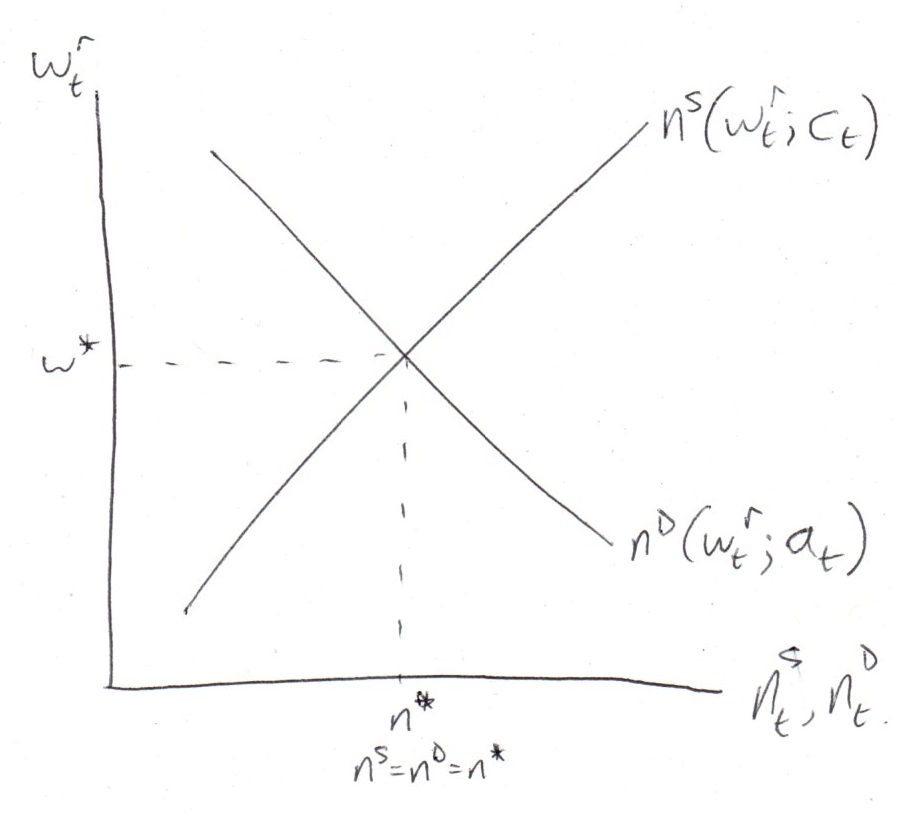
\includegraphics[width=0.7\textwidth]{Figures/lab_mkt_ns_f_c.jpg}}
\caption[Labor demand and supply]{\label{fig:lab_mkt_ns_f_c} Labor demand and supply}
\end{figure}

\end{frame}

%-------------------------------------------------------

%-------------------------------------------------------

\begin{frame}{Where's the `curve shifting'?}

In \textit{modern} macro, we must consider G.E. effects
	\begin{itemize}
	\item	Spillovers and interdependence
	\item	Multiple simultaneous directions of causality
	\item	Connections between variables required by aggregate/market clearing constraints
	\end{itemize}

\vspace{3mm}
Need to think \textit{very} carefully before shifting curves
	\begin{itemize}
	\item	Especially if we imagine shifting one in isolation
	\item	Why is it shifting?
	\item	What part of the state has changed?
	\end{itemize}

\end{frame}

%-------------------------------------------------------

%-------------------------------------------------------

\begin{frame}{Where's the `curve shifting'?}

In equilibrium, all endogenous variables in $t$ are functions of the state in $t$
\begin{itemize}
%\item	In our case, the state is $s_{t}\equiv(a_{t},z_{t})$ - if we know its value, we can say what happens in the current period in equilibrium
\item	Though we haven't yet solved for it, $c_{t} = c(s_{t})$ in equilibrium
\item	Note that the firm's labor demand only depends on $a_{t}$
\end{itemize}

\vspace{4mm}
Since household optimality $\Rightarrow$ desired labor supply depends on $a_{t}$ \textit{and} $c_{t}$ we can re-write the labor supply curve as a function of $w_{t}^{r}$ where its location in $(n_{t},w_{t}^{r})$ space depends on $s_{t}$
\[
n^{s}_{t} = \hat{n}^{s}(w_{t}^{r};s_{t}) \equiv n^{s}(w_{t}^{r};c(s_{t}))
\]

\end{frame}

%-------------------------------------------------------

%-------------------------------------------------------

\begin{frame}{Where's the `curve shifting'?}

\begin{figure}[!htb]
\center{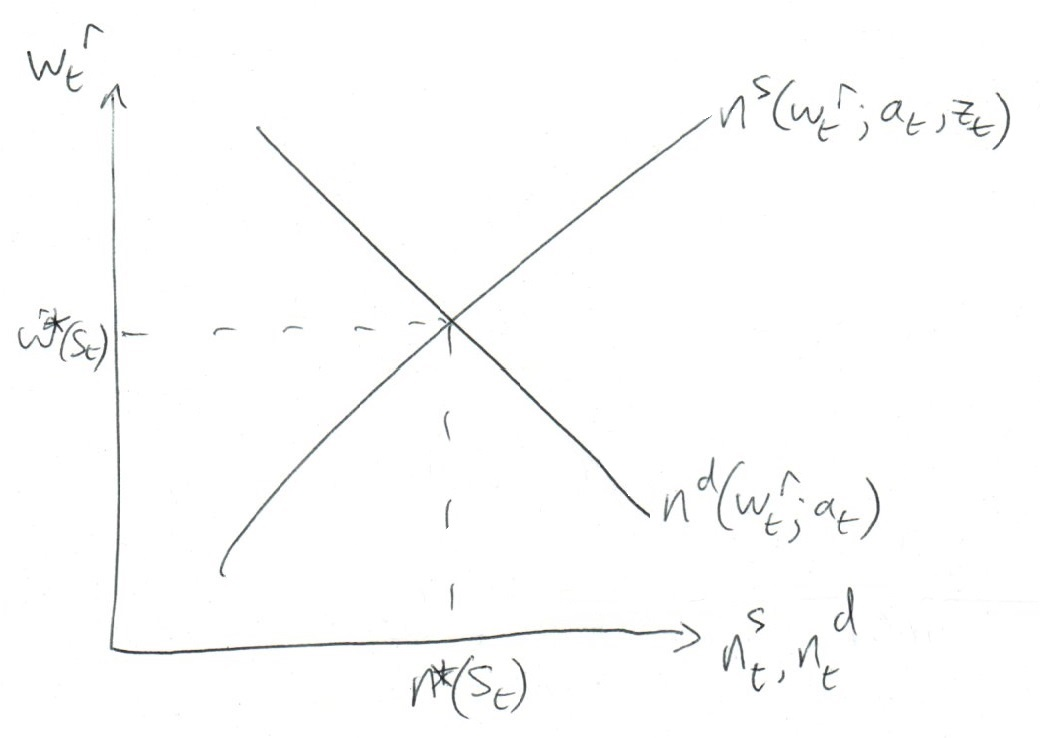
\includegraphics[width=0.7\textwidth]{Figures/lab_mkt.jpg}}
\caption[Labor demand and supply]{\label{fig:lab_mkt} Labor demand and supply}
\end{figure}

\end{frame}

%-------------------------------------------------------

%-------------------------------------------------------

\begin{frame}[label=curveshift]{Where's the `curve shifting'?}

In this simple model (keeping preference parameters etc. fixed) can you shift one curve and not the other?
\begin{itemize}
\item	No if it is $a_{t}$ that is changing
\item	(Maybe) yes if it is $z_{t}$ that is changing (only $n^{s}$ shifts - or does it\ldots?)
\end{itemize}

\vspace{2mm}
Finally, note that $w^{r}_{t}$ (the real wage) is also an equilibrium object
\begin{itemize}
\item	To find the function by which equilibrium $c_{t}$ depends on $s_{t}$ we will need to use other equations (mkt. clearing, production function etc.)
\item	Without that we can't find the intersection with the $n^{d}$ curve as the location of the labor supply curve is unknown
\item	You now see why I talk about solving a system of equations\ldots
\end{itemize}

\vspace{2mm}
\hyperlink{bachmann}{\beamerbutton{Bachmann \textit{et al} (2013)}}

\end{frame}

%-------------------------------------------------------

%-------------------------------------------------------

\begin{frame}{Competitive equilibrium}

Equilibrium requires that optimality conditions are respected but also\ldots
\begin{itemize}
\item	Decisions are consistent and feasible in aggregate
\item	Prices ensure that market clearing occurs
\end{itemize}

Initially we will only derive the equilibrium values of `real' variables
\begin{itemize}
\item	Consumption
\item	Output
\item	Employment
\item	Real wage
%\item	Real dividends
\item	Real savings
\item	Real interest rate
\end{itemize}

We will then model the nominal variables separately
\begin{itemize}
\item	Separation of real and nominal is a \emph{very} special aspect of this model
\item	Does not hold in NK model (that's the point\ldots)
\end{itemize}

\end{frame}

%-------------------------------------------------------

%-------------------------------------------------------

%\begin{frame}{Some additional variables}
%
%Real savings
%\begin{itemize}
%\item	Real value of bond purchases, $S^{r}_{t} \equiv \frac{Q_{n,t}B_{t}}{P_{t}}$
%\end{itemize}
%
%Real dividends
%\begin{itemize}
%\item	Real value of profits, $D^{r}_{t} \equiv \frac{D_{t}}{P_{t}} = Y_{t} - w^{r}_{t} n_{t}$
%\end{itemize}
%
%\end{frame}

%-------------------------------------------------------

%-------------------------------------------------------

\begin{frame}{Equilibrium conditions - real block}

\begin{description}
\item[1. Final good market clearing \textcolor{red}{(demand = supply)}] 			\hfill \\ 	$c_{t} = y^{s}_{t}$
\item[2. Labor market clearing \textcolor{red}{(demand = supply)}]				\hfill \\	$n^{d}_{t} = n^{s}_{t}$
\item[3. Aggregate final goods supply \textcolor{red}{(technical constraint)}]		\hfill \\	$y^{s}_{t} = a_{t} + \left( 1-\alpha \right)n^{d}_{t}$
\item[4. Labor supply \textcolor{red}{(optimality)}]	\hfill \\	$w^{r}_{t} = \sigma c_{t} + \varphi n^{s}_{t}$
\item[5. Labor demand \textcolor{red}{(optimality)}]	\hfill \\	$w^{r}_{t} = \log{\left( 1-\alpha \right)} + a_{t} - \alpha n^{d}_{t}$
\item[6. (Real) savings \textcolor{red}{(accounting)}]					\hfill \\	$S^{r}_{t} = \exp{(y^{s}_{t})} - \exp{(c_{t})}$
%\item[7. (Real) dividends \textcolor{red}{(accounting)}]					\hfill \\	$D^{r}_{t} =\exp{(y^{s}_{t})} - \exp{(w^{r}_{t} + n^{d}_{t})}$
\item[7. Euler equation \textcolor{red}{(optimality)}]	\hfill \\	$r_{t} = \rho + \left( 1-\rho_{z} \right) z_{t}+ \sigma E_{t} \left[ \Delta c_{t+1} \right]$
\end{description}

\end{frame}

%-------------------------------------------------------

%-------------------------------------------------------

\begin{frame}{Solving for the model's equilibrium - real block}

First we note that we can use market clearing to say
\begin{eqnarray*}
n^{s}_{t} 	= n^{d}_{t} \mathbf{= n_{t}} \\
c_{t}		= y^{s}_{t} \mathbf{= y_{t}}
\end{eqnarray*}
so we can just talk in terms of employment ($n_{t}$) and output ($y_{t}$)

\vspace{3mm}
Then we have
\begin{eqnarray}
y_{t} &=& a_{t} + \left( 1-\alpha \right) n_{t} \label{eqn:prod_fn} \\
w_{t} &=& \log{\left( 1-\alpha \right)} + a_{t} - \alpha n_{t} \label{eqn:lab_dem} \\
w_{t} &=& \sigma y_{t} + \varphi n_{t} \label{eqn:lab_supp}
\end{eqnarray}

\end{frame}

%-------------------------------------------------------

%-------------------------------------------------------

\begin{frame}{Solving for the model's equilibrium - real block}

Using equations (\ref{eqn:lab_dem}) and (\ref{eqn:lab_supp}) we obtain
\[
y_{t} = \frac{1}{\sigma} \left( \log{\left(1-\alpha \right)} + a_{t} -\left( \alpha + \varphi \right) n_{t} \right)
\]

Combining with equation (\ref{eqn:prod_fn}) $\Rightarrow n_{t}$ in terms of exogenous variables
\begin{eqnarray}
\textcolor{red}{n_{t}}	&\textcolor{red}{=}& \textcolor{red}{\psi_{n} + \psi_{n,a} a_{t}} \label{eqn:n_classical}\\
\psi_{n} &\equiv& \frac{\log{\left( 1 - \alpha \right)}}{\left( 1 - \alpha \right) \sigma + \alpha + \varphi} \nonumber \\
\psi_{n,a} &\equiv& \frac{1-\sigma}{\left( 1 - \alpha \right) \sigma + \alpha + \varphi} \nonumber 
\end{eqnarray}

Substituting back into equation (\ref{eqn:prod_fn}) yields
\begin{eqnarray}
\textcolor{red}{y_{t}}	&\textcolor{red}{=}& \textcolor{red}{\psi_{y} + \psi_{y,a} a_{t}} \label{eqn:y_classical} \\
\psi_{y} &\equiv& \left( 1-\alpha \right) \psi_{n}  \nonumber \\
\psi_{y,a} &\equiv& \frac{1+\varphi}{\left( 1 - \alpha \right) \sigma + \alpha + \varphi}  \nonumber 
\end{eqnarray}

\end{frame}

%-------------------------------------------------------

%-------------------------------------------------------

\begin{frame}{Solving for the model's equilibrium - real block}

We can use the labor supply condition, goods market clearing and the equilbrium expression for $n_{t}$
to obtain
\begin{eqnarray*}
w_{t} 	&=& \sigma y_{t} + \varphi n_{t} \\
		&=& \sigma( \psi_{y} + \psi_{y,a} a_{t} ) + \varphi (\psi_{n} + \psi_{n,a} a_{t})
\end{eqnarray*}

So we obtain\ldots
\begin{eqnarray}
\textcolor{red}{w_{t}}	&\textcolor{red}{=}& \textcolor{red}{\psi_{w} + \psi_{w,a} a_{t}} \\
\psi_{w}	& \equiv & \frac{(\sigma(1-\alpha)+\varphi)\log{(1-\alpha)}}{\sigma(1-\alpha)+\varphi + \alpha} \nonumber \\
\psi_{w,a} &\equiv& \frac{\sigma + \varphi}{(1-\alpha)\sigma+\alpha+\varphi} > 0 \nonumber
\end{eqnarray}

\end{frame}

%-------------------------------------------------------

%-------------------------------------------------------

\begin{frame}[label=wageresponse]{Solving for the model's equilibrium - real block}

\[
\psi_{n,a} \equiv \frac{1-\sigma}{\left( 1 - \alpha \right) \sigma + \alpha + \varphi}
\]
Income effect (through $c\uparrow$) vs. substitution effect (through $w\uparrow$) 
\begin{itemize}
\item	$\sigma \rightarrow 1$ (log utility) then $\psi_{n,a}\rightarrow 0$
\item	$\sigma > 1 \Leftrightarrow EIS < 1 \Leftrightarrow \psi_{n,a} <  0$
\item	$\sigma < 1 \Leftrightarrow EIS > 1 \Leftrightarrow \psi_{n,a} > 0$
\item	Income (substitution) effect dominates with $ EIS <(>) 1$
\item	\hyperlink{utfn}{Strength of response attenuated as $\varphi \uparrow$}
\end{itemize}

\[
\psi_{y,a} \equiv \frac{1+\varphi}{\left( 1 - \alpha \right) \sigma + \alpha + \varphi} > 0
\]
If $\sigma \rightarrow 1$ (log utility) then $\psi_{y,a}\rightarrow 1$
\begin{itemize}
%\item	Follows from specification of production function and $\psi_{n,a}\rightarrow 0$
\item	Only change in output must come from $a_{t}$ without any $n_{t}\uparrow$
\end{itemize}

\end{frame}

%-------------------------------------------------------

%-------------------------------------------------------

\begin{frame}{Solving for the model's equilibrium - real block}

\[
\psi_{w,a} \equiv \frac{\sigma + \varphi}{(1-\alpha)\sigma+\alpha+\varphi} > 0
\]

Wages are pro-cyclical under technology-induced fluctuations
\begin{itemize}
\item	Both $\psi_{y,a}$ and $\psi_{w,a}$ are positive
\end{itemize}
%Note that as $\sigma \rightarrow 1$ (log utility) $\psi_{w,a} \rightarrow 1$
%\begin{itemize}
%\item	Unit elasticity of wage to technology
%\item	Also, note that $\psi_{w,a} \uparrow $ as $\sigma \uparrow$
%\item	So if EIS is less (more) than unity, $\psi_{w,a}$ more (less) than unity
%\end{itemize}

\vspace{2mm}
It is immediate to obtain expressions for other variables (setting aside $r_{t}$)
\begin{itemize}
%\item	$w^{r}_{t}$: Use the labor supply condition and expression for $n_{t}$
\item	$c_{t}$: We have $c_{t}=y_{t}$ so same as for $y_{t}$
%\item	Dividends follow from simple accounting
\item	Savings follow from simple accounting
\end{itemize}

\end{frame}

%%-------------------------------------------------------
%
%%-------------------------------------------------------
%
%\begin{frame}{Solving for the model's equilibrium - real block}
%
%Technical side notes (\textbf{you can probably ignore this\ldots})
%\begin{itemize}
%\item	So far, all these variables have been calculated exactly
%\item	We converted some to log form, but no approximations yet used
%	\begin{itemize}
%	\item	Haven't yet used the log-linearized intertemporal optimality condition
%	\item	Avoid \textbf{log} dividends as that would need approximation for log-linearity
%	\[
%	\log{D^{r}_{t}} = \log{(Y_{t} - W^{r}_{t}N_{t})} \neq y_{t} - w^{r}_{t} - n_{t}
%	\]
%	\item	$S_{t}=0$ means it doesn't make sense to use logs anyway
%	\end{itemize}
%\item	This simplicity is very rare - most models need almost everything approximated
%\end{itemize}
%
%\end{frame}

%-------------------------------------------------------

%-------------------------------------------------------

\begin{frame}{Solving for the model's equilibrium - real block}

Note that $S^{r}_{t} \equiv \frac{Q_{n,t}B_{t}}{P_{t}}=0$
\begin{itemize}
\item	Real value of nominal bond holdings is zero
\item	Assuming positive prices, this implies $B_{t}=0$
\item	Identical households means no one holds bonds \textbf{in equilibrium}
	\begin{itemize}
	\item	All households have same optimality conditions
	\item	If \emph{anybody} wants to save, then \emph{everybody} wants to save!
	\item	Not feasible because no one takes the other side of the trade
	\end{itemize}
\end{itemize}

\vspace{2mm}
Sort of obvious from the start - why?
\begin{itemize}
\item	No way to transfer resources to future \emph{in aggregate}
\item	Other models: possible via investment in `capital' or foreign borrowing
\end{itemize}

\vspace{2mm}
\textbf{Equilibrium requires optimality *and* feasibility}

\end{frame}

%-------------------------------------------------------

%-------------------------------------------------------

\begin{frame}{Solving for the model's equilibrium - real block}

This is one way of seeing that, despite appearances, we could have guessed earlier that the aggregate $n^{s}$ curve would not depend on $z_{t}$
\begin{itemize}
\item	Imposing $c_{t}=y_{t}$ and rearranging the labor supply condition (to get the supply curve)
\end{itemize}
\begin{eqnarray*}
n_{t}^{s} 	&=& \frac{1}{\varphi}w_{t} - \frac{\sigma}{\varphi}c_{t} \\
			&=& \frac{1}{\varphi}w_{t} - \frac{\sigma}{\varphi}y_{t}
\end{eqnarray*}
\begin{itemize}
\item	From firm optimality, labor demand is only going to depend on $a_{t}$
\item	But, in equilibrium, labor demand pins down output, $y_{t}$, through the production function
\end{itemize}

\vspace{2mm}
So the curves can't be shifted independently, even with a $z_{t}$ impulse
\end{frame}

%-------------------------------------------------------

%-------------------------------------------------------

\begin{frame}{Where's the `curve shifting'? - Revisited}

\begin{figure}[!htb]
\center{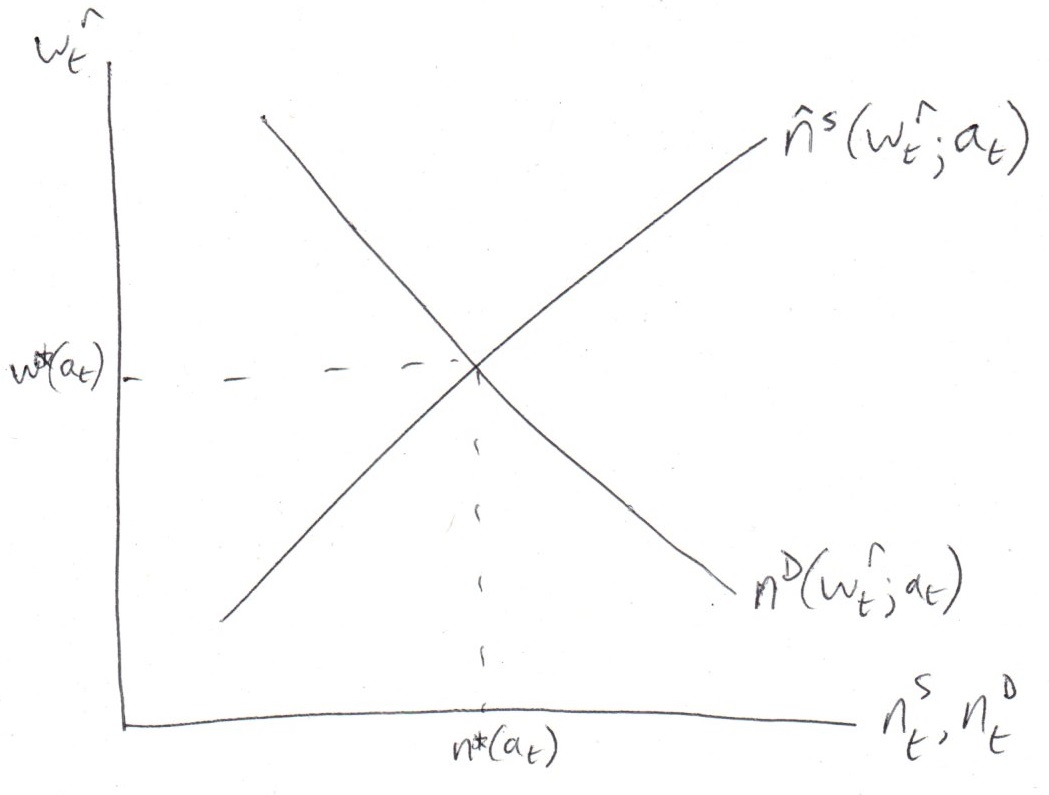
\includegraphics[width=0.7\textwidth]{Figures/lab_mkt_2.jpg}}
\caption[Labor demand and supply]{\label{fig:lab_mkt_2} Labor demand and supply}
\end{figure}

\end{frame}

%-------------------------------------------------------

%-------------------------------------------------------

\begin{frame}{Solving for the model's equilibrium - real block}

\begin{itemize}
\item	Households don't know/care about equilibrium
	\begin{itemize}
	\item	They just see prices and choose what's best for them individually
	\end{itemize}

\vspace{2mm}
\item	It is our \emph{assumption of equilibrium} (which must feature zero savings in this case) that pins down the necessary prices
	\begin{itemize}
	\item	How do these prices come about in a competitive model (where everyone is a price taker)?
	\item	Deep questions (see tatonnement, bargaining, the `core', \ldots)
	\item	In NK model, (goods) price setting is determined explicitly by firms' decisions
	\end{itemize}

\vspace{2mm}
\item	\emph{In equilibrium} prices must induce zero savings as optimal choice
	\begin{itemize}
	\item	$z_{t}$ affects the relative desirability of consumption today vs. tomorrow
	\item	$z_{t} \uparrow \Rightarrow$ people want to save less \emph{for a given $r_{t}$}
	\item	So $r_{t}$ must be a function of $z_{t}$ in equilibrium
	\end{itemize}

\end{itemize}

\end{frame}

%-------------------------------------------------------

%-------------------------------------------------------

\begin{frame}{Solving for the model's equilibrium - real block}

Finally, we derive the equilibrium real interest rate using\ldots
\begin{itemize}
\item	Intertemporal optimality (Euler equation)
\item	$c_{t}=y_{t}$ (where zero savings most obviously gets incorporated)
\item	The `solution' for $y_{t}$
\item	AR(1) process for $a_{t}$
\end{itemize}
\begin{eqnarray*}
r_{t} &=& \rho + \left(1-\rho_{z}\right)z_{t} + \sigma E_{t}\left[ \Delta y_{t+1} \right] \\
	&=& \rho + \left(1-\rho_{z}\right)z_{t} - \sigma \left( 1-\rho_{a} \right) \psi_{y,a} a_{t} \\
	&\equiv& \psi_{r} + \psi_{r,a} a_{t} + \textcolor{red}{\psi_{r,z} z_{t}}
\end{eqnarray*}

In a `perfect foresight' steady state where $z_{t}=a_{t}=0$ we have
\[
r = \rho \equiv -\log{(\beta)}
\]

The steady state real interest rate is determined by time preference

\end{frame}


%-------------------------------------------------------

%-------------------------------------------------------

\begin{frame}{Solving for the model's equilibrium - real block}

At this point we have\ldots
\begin{itemize}
\item	Expressions of the form
\[
var_{t} = \psi_{var} + \psi_{var,a} a_{t} + \psi_{var,z} z_{t}
\]
for $var \in \{ c_{t}, y_{t}, n_{t}, w^{r}_{t}, r_{t} \}$
\item	Exact expressions for savings ($=0$)% and real dividends
\item	The AR(1) specifications for $a_{t}$ and $z_{t}$ 
\end{itemize}

\vspace{3mm}
These components constitute the `solution' of the real side of the model for all the real variables of interest

\end{frame}

%-------------------------------------------------------
\section{Equilibrium - Nominal block}
%-------------------------------------------------------

\begin{frame}

\begin{center}
{\LARGE Equilibrium - Nominal Block}
\end{center}

\end{frame}

%-------------------------------------------------------

%-------------------------------------------------------

\begin{frame}{Solving for the model's equilibrium - nominal block}

\begin{itemize}
\item	The nominal aspects of the model have no implications for the behavior of real variables
\item	As such, they are irrelevant for welfare and imply no role for policy
\item	Nevertheless it is useful to consider how the behavior of $P_{t}$ depends on monetary policy
\item	Policy is captured by a rule for the \emph{nominal} interest rate $i_{t}$
\end{itemize}

\end{frame}

%-------------------------------------------------------

%-------------------------------------------------------

\begin{frame}{Solving for the model's equilibrium - nominal block}

Recall the Fisher equation
\[
i_{t} = r_{t} + E_{t}[ \pi_{t+1} ]
\]

In this model, $r_{t}$ is already pinned down on the real side
\begin{itemize}
\item	$\Rightarrow$ conditional on $r_{t}$, inflation expectations and $i_{t}$ move 1:1
\item	This applies in the short run (not simply \emph{long run} Classical dichotomy)
\end{itemize}

\vspace{3mm}
For a given steady state rate of inflation, $\pi$ we can thus obtain the associated steady state value of $i_{t}$
\[
i = \rho + \pi
\]
since (recall) $r_{t}=\rho$ in steady state

\end{frame}

%-------------------------------------------------------

%-------------------------------------------------------

\begin{frame}{Solving for the model's equilibrium - nominal block}

Let us consider a simple policy rule for $i_{t}$
\begin{eqnarray*}
i_{t} 	&=& \rho + \pi + \phi_{\pi} (\pi_{t}-\pi) + v_{t} \\
		&=& r + \pi + \phi_{\pi} (\pi_{t}-\pi) + v_{t}
\end{eqnarray*}
where $\phi_{\pi}>0$ determines the strength of the response of policy to deviations in inflation from $\pi$

\vspace{2mm}
$v_{t}$ is a policy `shock' that follows an AR(1)
\begin{eqnarray*}
v_{t} 				&=& 					\rho_{v} v_{t-1} + \varepsilon_{t}^{v} \\
\varepsilon_{t}^{v}	&\stackrel{iid}{\sim}&	 N\left(0,\sigma_{v}^{2}\right)
\end{eqnarray*}

\vspace{1mm}
What is $v_{t}$?
\begin{itemize}
\item	A random, temporary deviation from `usual' policy conduct
\item	Note: In recent years $v_{t}$ likely have become `smaller' (Ramey 2016)
\end{itemize}

\end{frame}

%-------------------------------------------------------

%-------------------------------------------------------

\begin{frame}{Solving for the model's equilibrium - nominal block}

If we subtract the policy rule from the Fisher equation we obtain (where we define $\hat{\pi} \equiv \pi_{t}-\pi$ and $\hat{r} \equiv r_{t}-r$)
\[
\hat{\pi}_{t} = \frac{1}{\phi_{\pi}} E_{t}[\hat{\pi}_{t+1}] + \frac{1}{\phi_{\pi}}\left(\hat{r}_{t} - v_{t}\right)
\]

If $\phi_{\pi}>1$ then (under reasonable assumptions) we can solve for
\[
\hat{\pi}_{t} = \sum\limits_{k=0}^{\infty} \phi_{\pi}^{-(k+1)}E_{t}\left[ \hat{r}_{t+k} - v_{t+k} \right]
\]

Given our earlier solution for $r_{t}$ in equilibrium and the assumed processes for $a_{t}$, $z_{t}$ and $v_{t}$ we can rewrite this as
\[
\hat{\pi}_{t} = \frac{\sigma(1-\rho_{a})\psi_{ya}}{\phi_{\pi} - \rho_{a}} a_{t} + \frac{1-\rho_{z}}{\phi_{\pi} - \rho_{z}} z_{t} - \frac{1}{\phi_{\pi}-\rho_{v}} v_{t}
\]

\end{frame}

%-------------------------------------------------------

%-------------------------------------------------------

\begin{frame}{Solving for the model's equilibrium - nominal block}

With a solution for (an) equilibrium process for $\pi_{t}$ (equivalently, $\hat{\pi}_{t}$) the process for prices arises from
\[
p_{t} \equiv p_{t-1} + \pi_{t}
\]
which allows the conversion of real wages to nominal

\vspace{2mm}
Under $\phi_{\pi}>1$ this is the \emph{only} solution for the nominal elements of equilibrium
\begin{itemize}
\item	Under $\phi_{\pi}<1$ we have `equilibrium indeterminacy'
\item	Multiple equilibria are possible with the same `real' block but with different processes for inflation
\item	Hints that may be desirable to keep $\phi_{\pi}>1$ (the `Taylor principle')
	\begin{itemize}
	\item	But in \emph{this} economy \emph{all} the equilibria are welfare-equivalent since consumption and employment are the same
	\end{itemize}
\end{itemize}

\end{frame}

%-------------------------------------------------------
\section{Summary}
%-------------------------------------------------------

\begin{frame}

\begin{center}
{\LARGE Summary}
\end{center}

\end{frame}

%-------------------------------------------------------

%-------------------------------------------------------

\begin{frame}{Summary}

\begin{itemize}
\item	The model we have described has various unrealistic implications
	\begin{itemize}
	\item	In particular there is no role for monetary policy to influence the economy as empirical evidence suggests it should
	\item	Price setting is left undefined - in contrast to real world experience of sticky prices etc.
	\item	There is also no reason for policy to intervene, given efficiency of allocations
	\end{itemize}
\vspace{2mm}	
\item	However, it has allowed us to introduce various concepts
	\begin{itemize}
	\item	General equilibrium
	\item	Multiple sectors (households and firms)
	\item	Monetary policy `rule' for $i_{t}$
	\end{itemize}
\vspace{2mm}	
\item	We now move to the New Keynesian framework which is conceptually richer and empirically more successful
\end{itemize}

\end{frame}
